\documentclass{report}
\usepackage{graphicx} % Required for inserting images
\usepackage{indentfirst}
\usepackage[OT1,T1]{fontenc}
\usepackage{geometry}
\geometry{hmargin=2.5cm,vmargin=1.5cm}
\renewcommand{\thesection}{\arabic{section}}
\bibliographystyle{unsrt}
\usepackage[french]{babel}
\usepackage{sidecap}

\begin{document}
\begin{titlepage}



\newcommand{\HRule}{\rule{\linewidth}{0.5mm}} % Defines a new command for the horizontal lines, change thickness here

\center % Center everything on the page

\includegraphics[scale=0.8]{Images/logo.png}\\[1cm] % Include a department/university logo - this will require the graphicx package

\includegraphics[scale=0.8]{Images/logo_inrae.jpg}\\[1cm] % Include a department/university logo - this will require the graphicx package
\textsc{\Large Conception d'un projet de recherche et de développement}\\[0.5cm] % Major heading such as course name

\HRule \\[0.4cm]
{ \huge \bfseries Cahier des charges du projet : Analyse de données RNA-seq (champignons \textit{Fusarium})}\\[0.4cm] % Title of your document
\HRule \\[1.5cm]
 
% If you don't want a supervisor, uncomment the two lines below and remove the section above
\Large \emph{Clients:}\\
Nadia \textsc{Ponts}\\
Fabien \textsc{Dumetz}\\[1cm]

\Large \emph{Laboratoire:}\\
Laboratoire Bordelais de Recherche en Informatique\\[1cm]

\Large \emph{Auteurs:}\\
Djemilatou \textsc{Ouandaogo}\\
Linda \textsc{Khodja}\\
Lucien \textsc{Piat}\\
Maroa \textsc{Alani}\\[1cm]

\Large \emph{Superviseur:}\\
 Marie \textsc{Beurton-Aimar}\\[1cm]

\vfill % Fill the rest of the page with whitespace
\end{titlepage}


\tableofcontents
\newpage

\chapter{Introduction}

L'INRAE, ou Institut national de recherche pour l'agriculture, l'alimentation et l'environnement, est un organisme public de recherche français. En son sein,  l’unité de recherche Mycologie et Sécurité des Aliments cherche à comprendre les mécanismes de contamination des aliments par les mycotoxines. \cite{inrae} \\

Les champignons du genre Fusarium infectent le blé et produisent des toxines sur les épis destinés à la consommation. Ces derniers élevés en coculture forment un Meta organisme, le Meta-Fusarium. Ses composantes peuvent communiquer grâce à des petits ARN appelés smRNA. \\

La problématique du projet est d’analyser des données de smRNA-seq en sortie de séquenceurs short read Illumina, les aligner sur les génomes de référence, identifier les petits ARN produits dans chaque scénario de coculture et les quantifier.\\

Un pipeline de traitement sera produit par les étudiants du Master de Bio-informatique de Bordeaux pour répondre à la problématique et un rapport lui sera associé. \\

{\bf Mots-clés:} Fusarium, mycotoxines, coculture, Meta-Fusarium, communication, smRNA, RNAseq


\chapter{Analyse}
\section{Contexte}
\subsection{Contex biologique du genre \textit{Fusarium}}
Depuis un certain temps, les biologistes portent un vif intérêt aux champignons filamenteux du genre \textit{Fusarium}. En effet, les \textit{Fusarium} sont des phytopathogènes qui contaminent, entre autres, les céréales que consomme l’homme comme le blé. Chez ce dernier, ils entraînent la fusariose de l'épi qui détruit les cultures et entraîne des pertes économiques conséquentes. Ces mycètes, sont aussi à l’origine de la contamination des grains par des mycotoxines constituant un problème majeur de sécurité alimentaire. Ces toxines comme les B-trichothécènes sont très stables et se retrouvent dans les grains qui finiront dans l’alimentation.\\

\begin{SCfigure}[1][h]
    \centering
    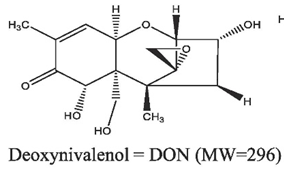
\includegraphics[width=0.25\textwidth]{Images/fig_1.png}
    \caption{Formule semi développée du Deoxynivalenol, molécule de la famille des B-trichothécènes produite par les \textit{Fusarium}\cite{gaballah2023development}}
    \label{fig:mol}
\end{SCfigure}

Jusqu’à lors, le processus de production des mycotoxines a été étudié en ne considérant "qu’un pathogène - une maladie". Cependant, des preuves irréfutables des interactions entre les espèces de \textit{Fusarium} responsables de la fusariose, laisse suggérer que la communication entre ces champignons puisse moduler la régulation de production des toxines.\\

Afin de mettre en exergue les mécanismes de production de ces molécules inter-individus, il est nécessaire changer d'échelle d'analyse d’observer plus globalement le " Meta-Fusarium sp."qui comprend les principales espèces impliquées dans l’infection.\cite{ponts2009fusarium, mycsa} \\

\begin{SCfigure}[1][h]
    \centering
    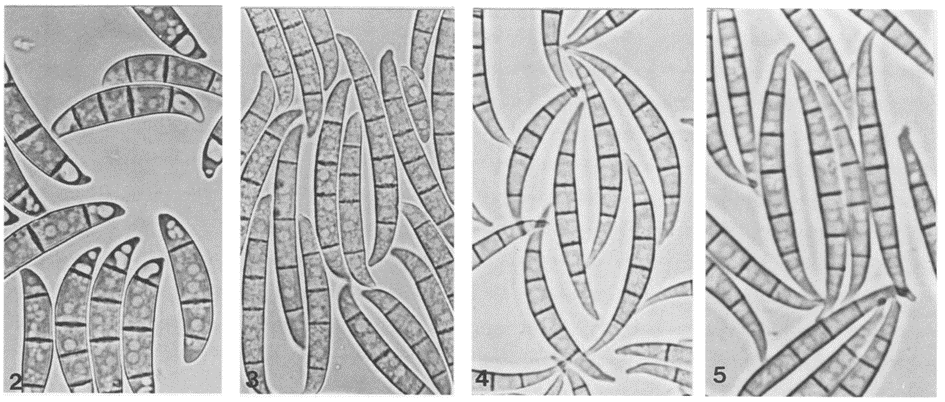
\includegraphics[width=.70\textwidth]{Images/fig_2.png}
    \caption{Observation des conidies de 2 : F.culmorum ; 3 : F.solani ; 4 : F.equiseti ; 5 : F.graminearum qui sont des champignons qui font partie du Meta-Fusarium sp. (950X) \cite{taxonomy}}
    \label{fig:fusa}
\end{SCfigure}

\subsection{La Communication au sein du Meta-Fusarium sp.}
Au sein du Meta-Fusarium sp. la communication s’effectue grâce à des petits acides ribonucléiques comme les small ARN (smRNA) ou les micro ARN (miRNA). Ces derniers sont des courtes suites de bases qui peuvent être séquencées.\\

\begin{figure}[h]
    \centering
    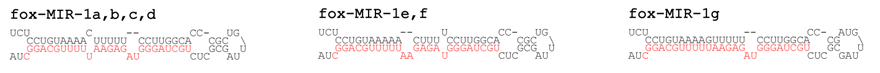
\includegraphics[width=1\textwidth]{Images/fig_3.png}
    \caption{Structure secondaire de quelques précurseurs miARN déjà mis en évidence chez les champignons du genre \textit{Fusarium}.\cite{chen2014exploring}}
    \label{fig:mirna}
\end{figure}

Ces petites molécules d'ARN non codantes d'environ 22 nucléotides, sont impliqués dans la régulation post-transcriptionnelle de l'expression génique. En identifiant les miARN spécifiques produits dans chaque scénario de co-culture et en comprenant leurs origines. Nous pourons mieux comprendre les mécanismes sous-jacents aux interactions hôte-pathogène et de développer des stratégies de prévention contre la contamination des cultures par les champignons \textit{Fusarium}. \cite{ponts2009fusarium, mycsa} \\

L’objectif du projet est d’analyser les données séquencées et d’identifier les microARN produits dans chaque scénario de culture, d’en repérer les spécificités et de les quantifier.

\section{Etat de l'art/Existant}
\subsection{Contrôle qualité des reads}
Contrôle qualité des fichiers fastQ pour supprimer ou modifier les artéfacts et les reads de mauvaise qualité.Utilisation de logiciels tels que FastQC. FastQC est un outil utilisé pour évaluer rapidement la qualité des données de séquençage. Il fournit des statistiques détaillées et des graphiques pour identifier les problèmes potentiels tels que la qualité des bases, la distribution des tailles d'insertion, la présence d'adaptateurs, etc.
FastQC est souvent utilisé comme première étape dans l'analyse des données de séquençage pour évaluer rapidement la qualité globale des échantillons. Il est gratuit est disponible
sur Github.\cite{fastqc}
Il existe un autre outil utilisé MultiQC \cite{multiqc} qui est un outil qui permet d'agréger les résultats de plusieurs analyses FastQC (ou d'autres outils similaires) en un seul rapport.MultiQC est particulièrement pratique lorsque vous effectuez une analyse à grande échelle impliquant de nombreux échantillons, car il permet de consolider les résultats de manière efficace.
Le choix entre FastQC et MultiQC dépend de notre besoin d'une évaluation détaillée de la qualité des données pour chaque échantillon individuel, ce qui signifie que FastQC est souvent le meilleur choix.

\subsection{Nettoyage des reads}
Trimmomatic \cite{trimmomatic}  est un outil largement utilisé pour nettoyer les reads en éliminant les bases de faible qualité, en coupant les adaptateurs et en éliminant les séquences de mauvaise qualité à partir des extrémités des reads.
 Trimmomatic produit des fichiers de sortie contenant les reads nettoyés, prêts à être utilisés pour l'alignement ou d'autres analyses. Il existe un autre outil utilisé Cutadapt \cite{martin2011cutadapt}  Il est également capable de détecter et de supprimer les régions de faible qualité, mais sa principale force réside dans la gestion précise des adaptateurs.Nous préférons Trimmomatic pour sa facilité d'utilisation et sa capacité à nettoyer rapidement les données de séquence.
 

\subsection{Alignement des reads sur le genome}
Bowtie2 \cite{bowtie2} est un outil de cartographie de reads à haut débit qui aligne efficacement les reads sur un génome de référence en utilisant l'algorithme de l'alignement parfaite. Il génère des fichiers d'alignement indiquant où chaque read s'aligne sur le génome de référence.BWA \cite{li2009fast} est un autre outil largement utilisé pour l'alignement de séquences d'ADN à courte lecture.Bowtie2 est généralement plus rapide que BWA, ce qui peut être bénéfique pour les analyses de séquençage d'ARN à grande échelle avec un grand nombre d'échantillons.

\subsection{Identification des petits ARN produits }
À partir des données de smRNA-seq, l'objectif est d'identifier les petits ARN (micro ARN - miARN) présents dans chaque échantillon issu de différentes situations de co-culture.Utilisation d'outils spécialisés comme miRDeep2 \cite{friedlander2012discover} ou miRBase \cite{kozomara2019mirbase} pour détecter et annoter les petits ARN dans les données alignées.MiRDeep2 est un outil spécifiquement conçu pour la prédiction de nouveaux microARN (miARN) à partir de données de séquençage.Il utilise à la fois les données de séquençage des petites ARN et les informations sur la structure secondaire des précurseurs de miARN pour prédire de nouveaux miARN et évaluer leur fiabilité.Mais MiRBase est une base de données de référence qui répertorie les séquences de miARN connues.MiRDeep2 est souvent utilisé lorsque l'on souhaite identifier de nouveaux miARN dans des données de séquençage, nous allons donc l'utiliser.

\subsection{Quantification des petits ARN }
Estimation des niveaux d'expression des petits ARN détectés à l'aide d'outils comme HTSeq\cite{anders2015htseq} ou featureCounts\cite{liao2014featurecounts}.HTSeq est un package Python conçu pour analyser les données de séquençage à haut débit, y compris les petites données de séquençage d'ARN.featureCounts fait partie du package Subread, qui fournit des outils pour cartographier et quantifier les lectures de séquences à partir d'expériences de séquençage à haut débit.Semblable à HTSeq, featureCounts prend en entrée des lectures de séquence alignées (au format BAM) et un fichier d'annotation de référence. Il attribue chaque lecture alignée à des caractéristiques génomiques spécifiées dans le fichier d'annotation, telles que des gènes ou de petits loci d'ARN.La sortie de featureCounts est également une matrice de comptage, où chaque ligne représente une caractéristique génomique et chaque colonne représente un échantillon, avec des valeurs indiquant le nombre de lectures mappées à chaque caractéristique dans chaque échantillon.Et featureCounts offre des options de comptage de lectures spécifiques à un brin, ce qui peut être important pour quantifier avec précision l'expression des petits ARN, en particulier en présence d'une transcription antisens.C’est donc l’option la plus appropriée.

\subsection{Analyse différentielle}
Identification des petits ARN différentiellement exprimés entre les différentes conditions de co-culture à l'aide d'outils comme DESeq2 \cite{love2014moderated} ou edgeR\cite{robinson2010edger}.DESeq2 et edgeR sont tous deux des outils bioinformatiques largement utilisés pour effectuer une analyse d’expression différentielle des données de séquençage d’ARN.Ils sont particulièrement utiles pour identifier des gènes ou d’autres caractéristiques génomiques qui présentent des différences d’expression statistiquement significatives entre différentes conditions expérimentales.

\subsection{Visualition des resultats}
Matplotlib est une bibliothèque de visualisation de données pour Python. Elle offre une grande variété de graphiques et de styles pour représenter les données, ce qui en fait un choix populaire pour la visualisation de données génomiques. Matplotlib permet de créer une grande variété de graphiques, y compris des histogrammes, des graphiques linéaires, des diagrammes en boîte, etc., pour représenter vos données de manière visuelle. Les visualisations produites avec Matplotlib peuvent être utilisées pour comprendre et présenter les résultats de l'analyse de séquençage, faciliter la communication des résultats ou guider les analyses ultérieures.\\


Tous les outils mentionnés peuvent être utilisés depuis Python via des interfaces ou des bibliothèques Python. Pour les outils FastQC, Trimmomatic et Bowtie2, l'importation de la bibliothèque subprocess permet leur exécution. Matplotlib est une bibliothèque Python directe. Il peut être installé et importé dans les scripts Python pour créer des visualisations de données génomiques ou de séquençage.


\section{Analyse des besoins}

\subsection{Besoins fonctionnels}
Pour le prétraitement des données, les besoins comprennent :
\begin{itemize}
    \item Acquisition des données issues du séquençage Illumina (Short Read) générées à partir de différentes conditions de culture de Fusarium au format FASTQ.
    \item Prétraitement et nettoyage des données brutes afin d'éliminer les séquences de faible qualité et les erreurs techniques en réalisant un contrôle qualité des lectures.
    \item Normalisation des données si nécessaire.
\end{itemize}
Pour l'analyse des données, les besoins incluent :  
\begin{itemize}
 \item Alignement des lectures prétraitées sur les génomes de référence des souches de Fusarium.
    \item Identifier les miARNs, déterminer leur origine ou leur localisation génomique, et évaluer leur quantité.
    \item Analyse comparative des profils d'expression des microARN entre les échantillons de cultures pures et ceux des confrontations entre souches.
    \item Visualisation des résultats à travers des tableaux et des graphiques codifiés présentant les profils d'expression des miARNs dans les différentes conditions de culture.
\end{itemize}

\subsection{Besoins non fonctionnels}
\begin{itemize}
    \item Utilisation recommandée des langages de programmation adaptés à la bioinformatique, tels que Python, R et éventuellement Bash.
    \item Traitement efficace des données dans des délais raisonnables.
    \item Fiabilité et robustesse pour minimiser les risques de perte de données ou d'erreurs dans l'analyse.
    \item Intuitivité pour une utilisation aisée par les chercheurs non spécialisés en bioinformatique.
    \item Documentation claire et interfaces rationnelles pour faciliter la navigation et l'utilisation des fonctionnalités.
\end{itemize}

\subsection{Contraintes}
\begin{itemize}
    \item Utiliser des outils open source afin d'assurer la transparence, la réutilisabilité du système.
    \item Effectuer nos tâches dans un cadre à accès pseudo-restreint.
    \item (a confirmer) Proposer des solutions de visualisation compatibles et integrables avec les bases de données fonctionnelles existantes pour les champignons filamenteux.
\end{itemize}

\subsection{Ajouts optionnels}
\begin{itemize}
    \item Création d'une base de données pour stocker les résultats.
    \item Sauvegarde et reprise du processus d'analyse et reprise de l'analyse là où elle s'est arrêtée.
    \item Identification des cibles potentielles des miARNs dans les génomes des souches.
\end{itemize}


\chapter{Flux opérationnel}
Voici un diagramme reprenant les différents points à réaliser.
\begin{center}
    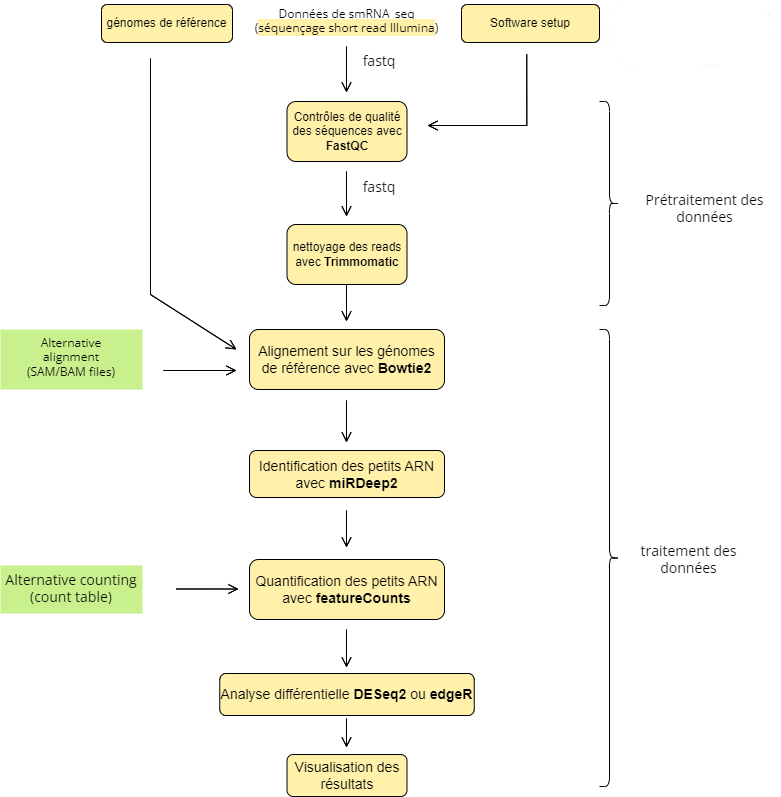
\includegraphics[scale=1.0]{Images/PIPLINE_RNA.png}\\[1cm]
\end{center}
\chapter{Organisation}
\section{Diagramme de Gantt}

\bibliography{biblio}

\end{document}